\documentclass[twocolumn,letterpaper]{article}

\usepackage{graphicx}
\usepackage{listings}
\usepackage{url}
\lstset{language=C}

\newcommand{\code}[1]{\texttt{#1}}

\title{SkyeFS: Distributed Directories using Giga+ and PVFS}
\author{Anthony Chivetta \url{<anthony@chivetta.org>}\\Swapnil Patil \& Garth
Gibson}
\date{DRAFT --- \today}

\begin{document}

\maketitle

\section{Overview}
PVFS, the Parallel Virtual File System, stores all metadata for a particular
directory on a single metadata server resulting in poor scalability in the case
of large or high traffic directories.  Giga+ is a scheme for partitioning the
metadata for a directory across a set of servers while still maintaining
performance for small directories..  SkyeFS implements the Giga+ algorithms on
top of an unmodified PVFS file system.

SkyeFS consists of a client (\code{skye\_\-client}) which functions as the
FUSE filesystem and a server (\code{skye\_\-server}) which provides
synchronization for metadata operations and controls directory placement and
splitting.  

Giga+ incrementally splits a directory into multiple partitions which are
load-balanced across available servers.  In SkyeFS, we represent each
partition as a distinct PVFS directory.  A SkyeFS server located with each
PVFS metadata server (MDS) provides the synchronization and coordination for
the partitions on the local PVFS MDS. 

\section{Implementation Overview}
We choose to implement Giga+ as an overlay filesystem on top of PVFS, instead
of modifying PVFS directly, in hopes of keeping the implementation small and
simple.  FUSE provides an obvious choice for implementing the client side of
the system due to the ease of writing a FUSE file system driver.
Additionally, the pvfs2\-fuse application distributed with the PVFS source
provides an example of how to implement FUSE operations in PVFS.  However,
unlike pvs2\-fuse, we use the lowlevel FUSE API.  This allows us to directly
specify the inode numbers returned to the kernel, avoiding extraneous pathname
resolution in the client by using PVFS handles as inode numbers.

In PVFS, every object is assigned a PVFS metadata handle and each PVFS server
is statically assigned a range of handles for which it is responsible.  
The directory entries in a directory are stored with that directory's metadata
on the server responsible for its metadata handle.  We exploit this property
of PVFS to manipulate metadata placement for each Giga+ partition.

\subsection{Physical Layout}
SkyeFS establishes a direct mapping between Giga+ partitions and a set of PVFS
directories.  This allows us to use Giga+ to both achieve load-balancing and
keep overall directory size small.  Rename operations in PVFS are relatively
cheep as they only move object metadata and not entire files.  This helps limit
the cost of any extra renames required by this storage scheme.  In systems
where this is not the case, a single directory per metadata server might be
used instead.

When a logical directory is created, we also create a PVFS directory on the
same server called ``p00000'' inside the logical directory to represent the
first Giga+ partition.  When this partition splits, a new directory ``p00001''
will be created adjacent to it to store the files in the new partition.  

The PVFS client uses round-robin assignment for selecting the metadata server
on which it will create a new  object.  Unfortunately, the PVFS client API
does not currently provide any way to influence this server selection.  When
creating PVFS directories for new partitions, we work around the problem by
repeatedly creating new directories until the resulting directory is on the
correct server.  Future versions of SkyeFS might cache these directories to
limit extraneous creates.

\subsection{Client/Server Architecture}
\begin{figure}
\begin{center}
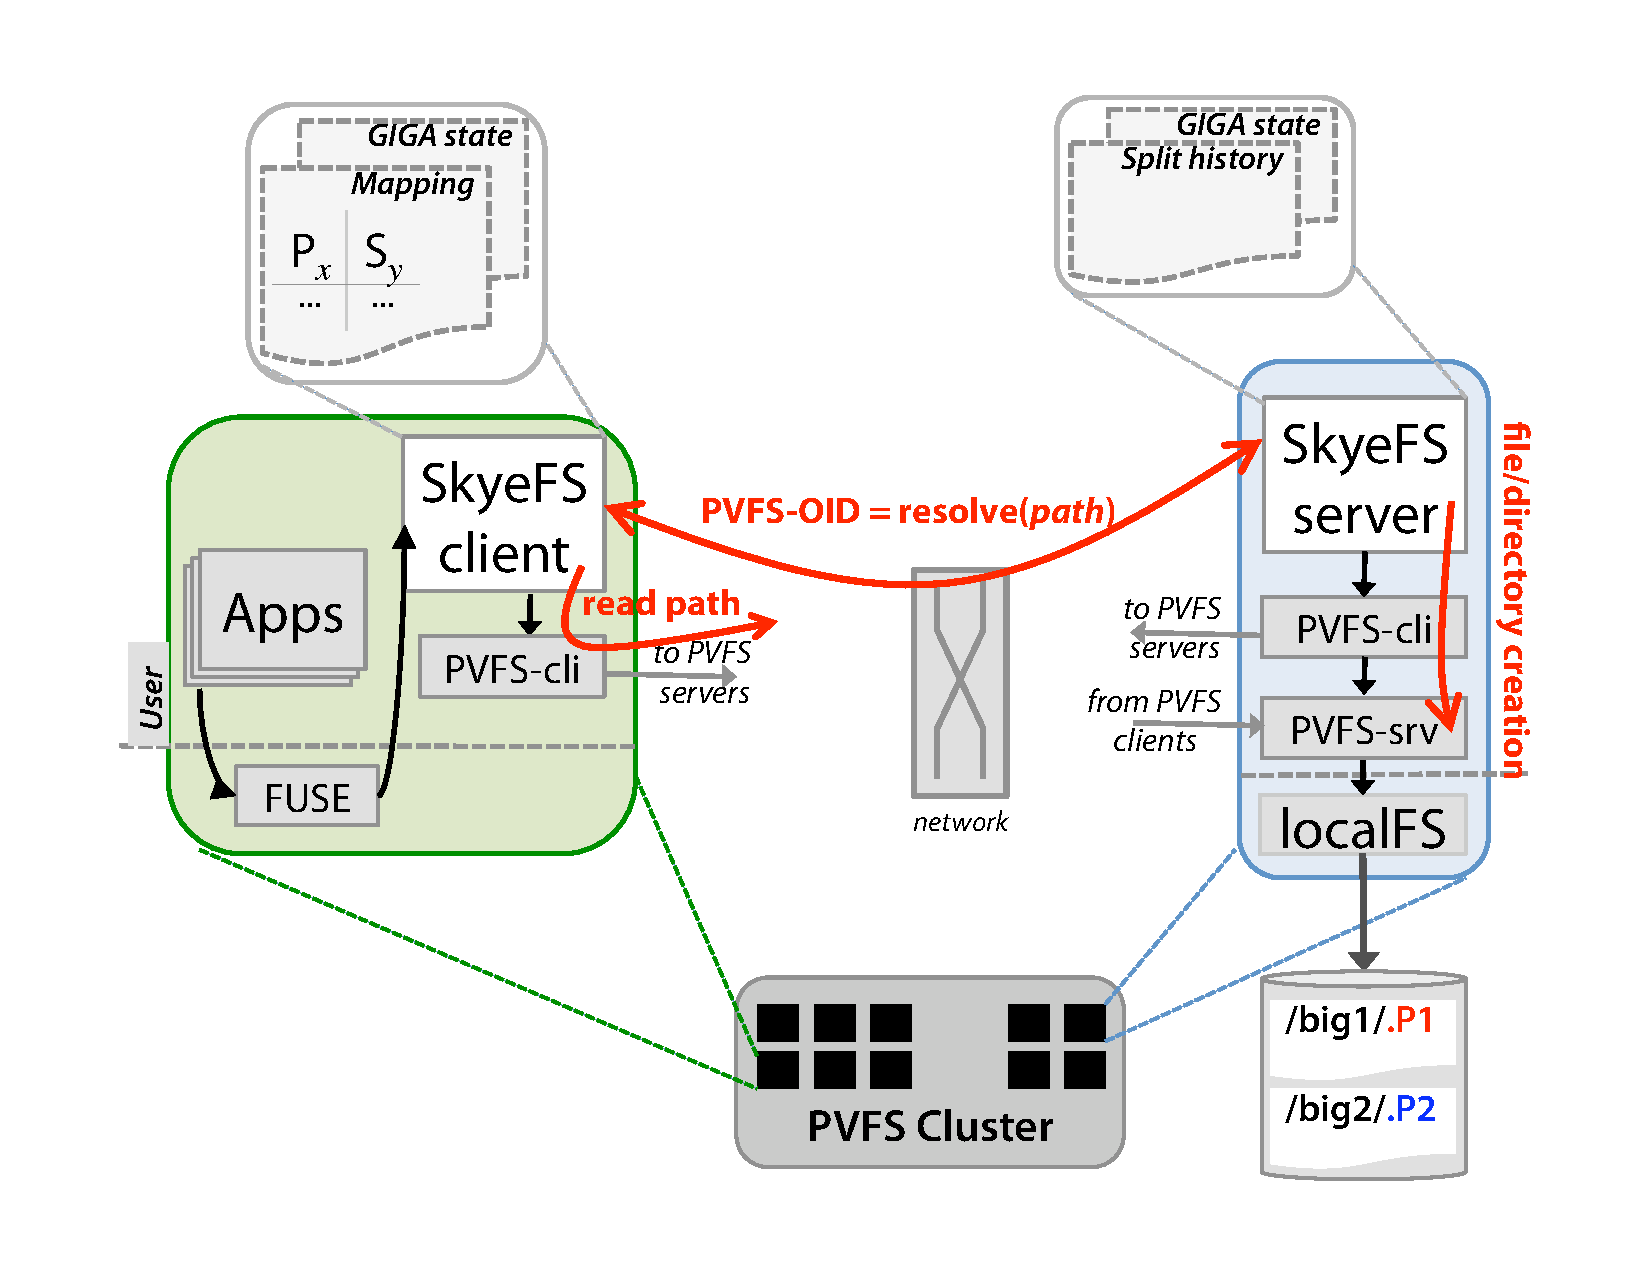
\includegraphics[width=3in]{figure-architecture}
\end{center}
\caption{SkyeFS Architecture Diagram}
\end{figure}

\begin{figure}
\begin{lstlisting}
struct skye_directory {
    giga_mapping mapping;
    int reference_count;
    PVFS_object_ref PVFS_handle;
    int splitting_index;
    pthread_rwlock_t rwlock;
    UT_hash_handle hashtable_handle;
};
\end{lstlisting}
\caption{Giga+ Directory Metadata}
\label{fig:skyedir}
\end{figure}

Giga+ has metadata that it must maintain in order to manage each directory's
partitions.  SkyeFS uses a small server process, \code{skye\_server}, located
on each PVFS server to manage this metadata and ensure consistency for the
directories and partitions resident on that server.  The \code{skye\_server}
has a cache of \code{skye\_directory} structures which store this metadata.
This metadata can be regenerated from PVFS at any time, allowing the
\code{skye\_server} to fail or evict items from its cache at any time without
the risk of leaving the system in an inconsistent state.

Each client runs a \code{skye\_client} process that provides a FUSE filesystem
and issues requests to the \code{skye\_server}s using ONC RPC and PVFS using
the PVFS system interface.  For most operations, the client is a simple
adaption of the \code{pvfs2-fuse} code to use the lowlevel FUSE API.  However,
metadata operations which require path name resolution or object creation are
forwarded through the \code{skye\_server} to prevent race conditions.  To
speed operation, the client also maintains a cache of the \code{giga\_mapping}
for recently accessed directories.

For performance and load-balance reasons, locality between the
\code{skye\_\-server} process and the PVFS server to which it is making
requests is maintained whenever possible.  Upon receiving a RPC request, the
server will first check if it owns the partition to be accessed by the
request.  If not, the server will return the error EAGAIN and provide
the client with a copy of its own mapping for the directory.  Upon receiving
this error, the client will read the server provided mapping and merge that
information with its local version.  The client will then reattempt the RPC
call to the new \code{skye\_\-server} as per the updated mapping.  This
ensures both that locality is maintained and that the client's cached mapping
will tend toward reality.

The most important job of the \code{skye\_server} is to prevent race
conditions during splitting.  Any operation that must resolve a pathname (such
as a lookup, create, or rename) needs to have an accurate Giga+ bitmap for the
directory so that they can operate on the correct partition.  By forwarding
these operations to the \code{skye\_server}, the server can ensure they happen
without interference from changing bitmaps.  There do exist schemes that would
allow client applications do so some of these operations without the server in
an optimistic manor; however, such schemes are error prone and overly
complicated.

\subsection{Path Resolution}
\begin{figure}
\begin{center}
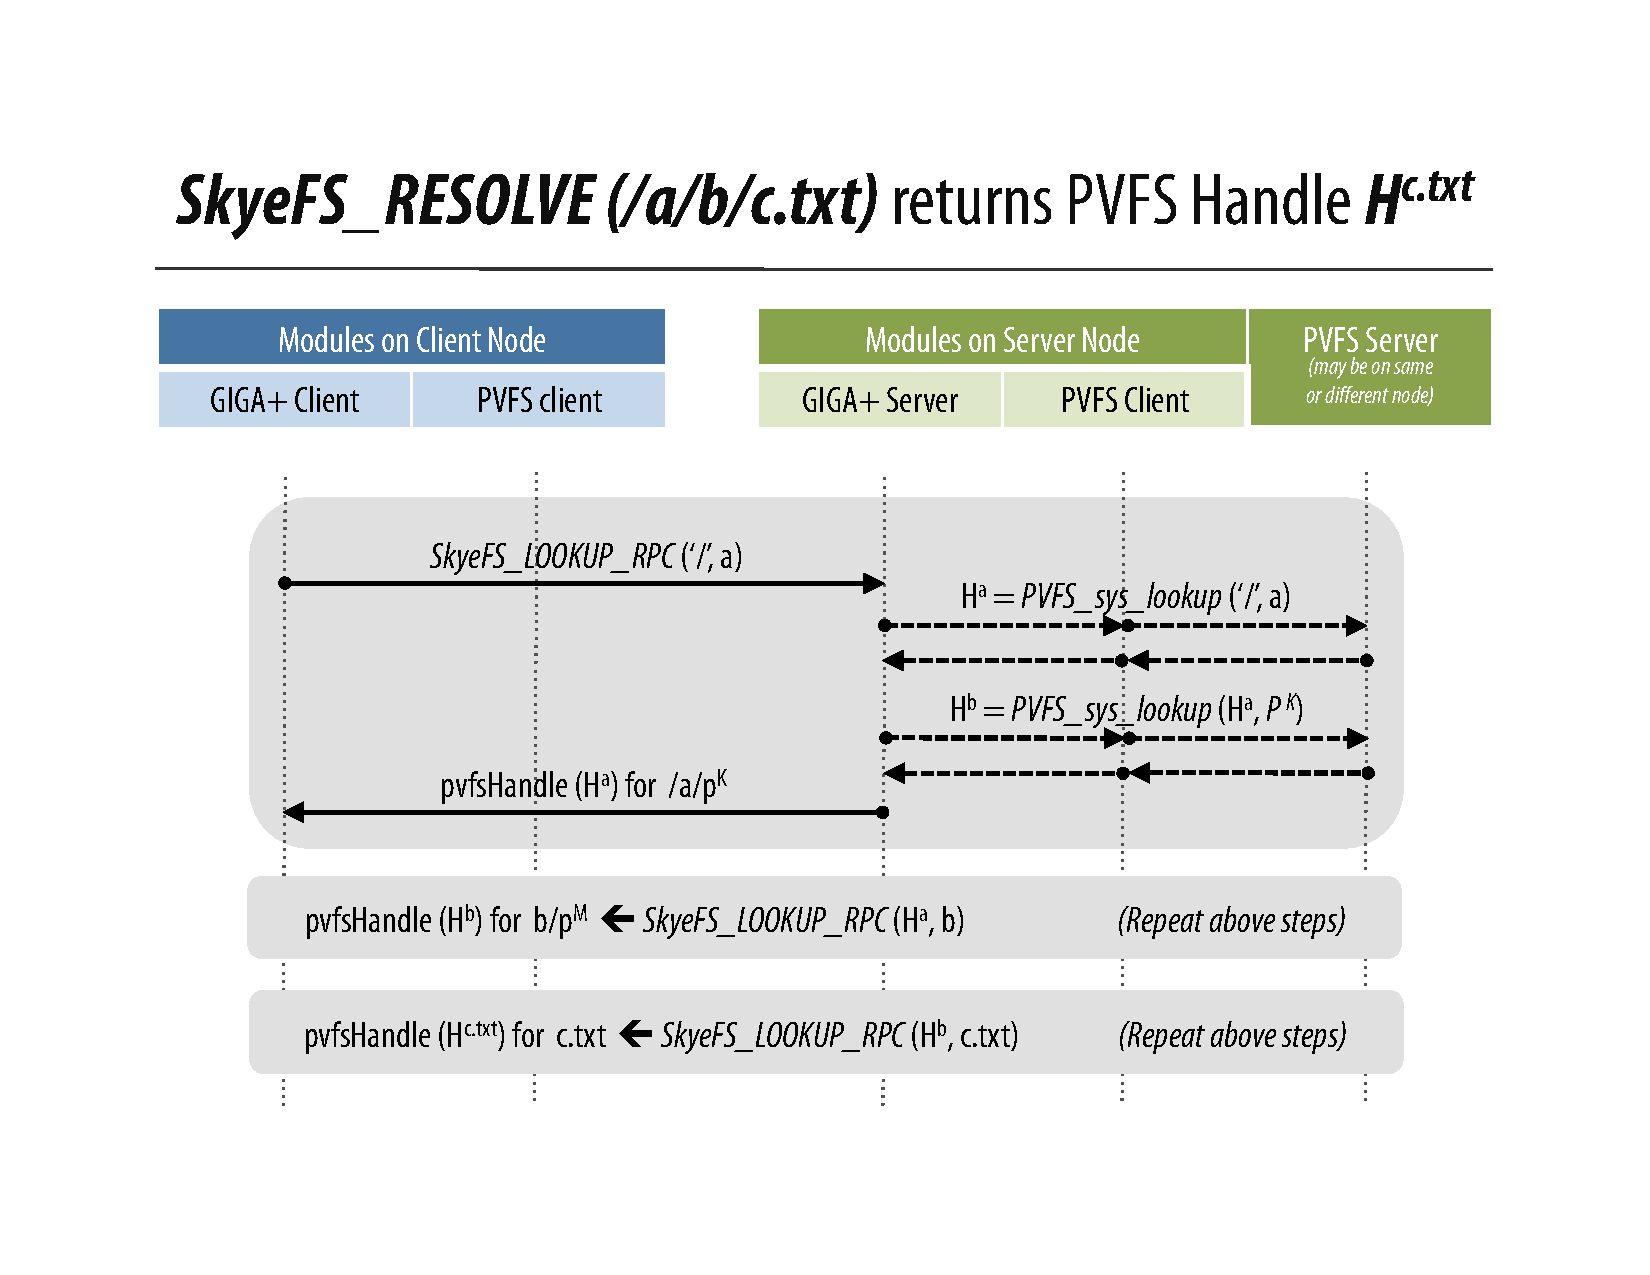
\includegraphics[width=3in]{figure-resolve}
\end{center}
\caption{SkyeFS Name Resolution}
\end{figure}
The FUSE lowlevel API uses a \code{lookup(inode, name)} callback to perform
path resolution.  We use the PVFS handle for an object as the FUSE inode to
avoid keeping a lookup table on the client.  PVFS provides a
\code{PVFS\_\-sys\_\-ref\_\-lookup(handle, name)} which is analogous to the
FUSE \code{lookup} function.  Our \code{skye\_server} wraps this PVFS function
to both resolve the Giga+ partition and the object itself and exposes an
\code{lookup} RPC to accomplish this.  When the \code{skye\_client} receives a
\code{lookup} callback, it consults its cached bitmap (if any) and then
makes an RPC call to the responsible \code{skye\_server}, retrying in the
event that an EAGAIN is returned.  By resolving both the partition and
requested object in the server, we avoid race conditions due to concurrent
splits.  \footnote{For example, issuing the RPC \code{lookup(NULL, ``foo'')}
would return the PVFS handle of ``/p00004/foo'' if ``foo'' was stored in the
fifth partition of the filesystem root.  If we let that handle be $h$, then
\code{lookup($h$, ``bar'')} would return the PVFS handle of
``/p00004/foo/p00002/bar'' if ``bar'' is in the third partition of ``foo''.
In this manor, any logical path can be resolved to its PVFS handle in a manor
opaque to the caller.}

As PVFS metadata handles do not change when their objects are moved between
directories, the handle returned by \code{lookup} is guaranteed to continue to
be a valid reference to the object for the duration of the object's existence.
This is true even if the partition holding an object splits or the logical
directory is moved elsewhere in the directory tree.  As a result, we can
safely return a PVFS handle to FUSE in the form of an inode umber.

\subsection{Metadata Persistence}
Closely related to the issue of physical layout is that of persisting SkyeFS
metadata.  This includes the Giga+ mapping (the bitmap and zeroth server), the
server list at the time of directory creation and the state of any splitting
directories.  To make the system as fault tolerant as possible, we avoid
explicitly storing any of this metadata and instead interrogate the state of a
directory in PVFS to determine these values.

Rather than building into SkyeFS our own mechanism for maintenance of server
lists we simply ask PVFS for the current server list on start up.  Tests indicate
that PVFS will always return this in the same order.  In the event of a server
addition the new servers are simply added to the end of the list.  As PVFS does
not support the removal of servers, we do not need to provide support for that
functionality.  Therefore, to determine the server list at the time of a
directory creation we only need to know the number of servers that existed when
the directory was created.

When the server's read-through cache suffers a cache miss it must populate a new
\code{struct skye\_\-directory} with the necessary information.  It determines
the zeroth server by asking PVFS for the MDS responsible for the directory's
PVFS handle.  It then performs a \code{readdir()} on the directory to find all
existing partitions (folders with the `p' prefix).  This also will reveal any
currently splitting partitions (folders with the `s' prefix).  If the server
determines that it is responsible for completing an unfinished split it will
enqueue the partition for completion by the split thread.\footnote{This is
currently unimplemented.} It will then read an extended attribute from the
directory that indicates the number of servers which existed when the
directory was created.\footnote{This is currently unimplemented.}  This
extended attribute is only ever written once, at the time the directory is
created, so there is no risk of inconsistency being introduced by directory
operations.  All the other values similarly do not face any inconsistency
risks as they are simply functions of the physical layout of the directory.

On the client side we use a significantly simplified version of the cache
population procedure to avoid hitting the PVFS servers.  When the read-through
cache suffers a miss it will simply create a new object with a bitmap consisting
of only the zeroth partition, a server list of length one and the zeroth server
set to the owner of the directory's handle.  The merging semantics of Giga+
mappings ensure that as the client receives updated mappings from the servers
this initial mapping will tend toward accurate.

Populating the initial mapping in this way causes the \code{lookup()} code to always
start with the zeroth server in the cache-cold state.  While this ensures that
some progress towards finding the correct server is always made, it has the
potential to cause unbalanced load on servers which act as the zeroth server for
popular directories.  One potential solution to this problem is to provide
bootstrapping hints to clients during the iterative \code{lookup()} process.
When a client performs a {lookup()} and the server detects that the object is
a directory the server should also return any cached bitmap it may have for
that directory to the client to populate its cache.  This would improve the
performance of cache-cold and cache-warm lookups by reducing the number of
servers a client must contact before it reaches the correct server. 

This persistence scheme results in a system that can halt at almost any time
without leaving the system in an inconsistent state.

\section{Filesystem Operations}
\subsection{Splitting and file creation}
\begin{figure}
\begin{center}
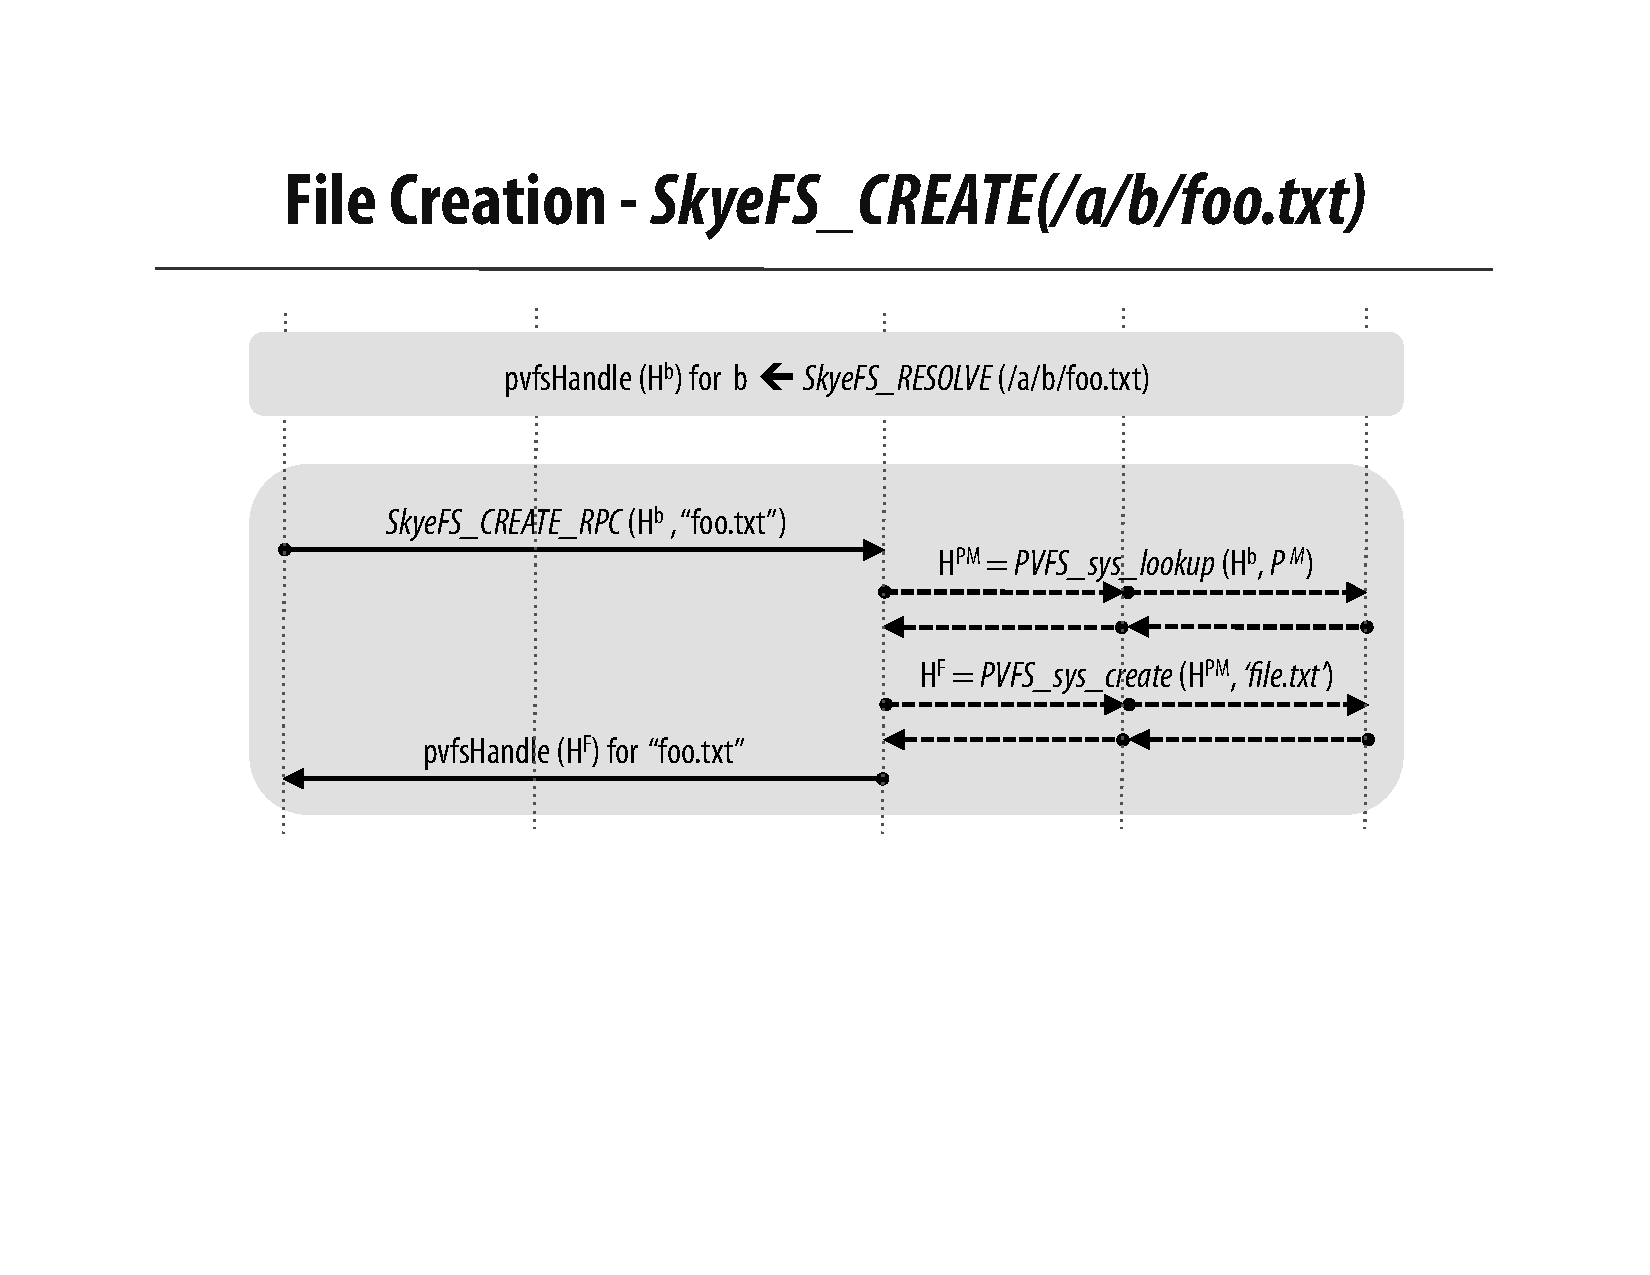
\includegraphics[width=3in]{figure-create}
\end{center}
\caption{SkyeFS Create Procedure}
\end{figure}
The \code{create()} RPC is used by \code{skye\_\-client} to create files in a given
directory.  Just like with \code{lookup()} only the server that owns the correct
partition for a file will service a \code{create()} call.  Quite simply, the
\code{create()} RPC calls \code{PVF\_\-sys\_\-create()} with the appropriate
parent handle.  The complex part is handling splitting during and after a
\code{create()}.

Splitting of partitions is a critical and potentially tricky part of the Giga+
algorithm.  In PVFS we are able to achieve a high degree of concurrency in the
face of splitting thanks to the stability of PVFS file handles and the rename
semantics.

Each logical directory is represented by a \code{struct skye\_\-directory} on
the server.  This structure is defined approximately as follows:


During normal operation, when no splits are happening,
\code{splitting\_\-index} has the value of -1.  When an operation needs to
access the directory, it acquires a read lock on the read-write lock for the
duration of the operation.  By holding the read-write lock, the operation can
be assured that no partition will begin to split until the lock is released.

At the end of the \code{create()} call, a \code{stat()} operation is performed
on the partition and the number of directory entries in the partition is
compared to the system's split threshold.  If the current directory size is
greater, the PVFS handle of the parent and the partition number are stored at
the end of a queue of partitions to split.  The \code{create()} call then
returns as normal.

Each \code{skye\_\-server} has a dedicated splitter thread.  This thread waits on a
condition variable associated with the split queue.  When an operation adds a
entry to the queue it signals on the condition variable to wake up the splitting
thread.  The splitting thread iterates through the queue and splits all
specified partitions which are found to still be over the splitting threshold.

To split a partition, the splitting thread first acquires a write lock in the
directory.  This ensures that all operations currently outstanding on the
directory are finished before the lock is acquired and that no new operations
may begin.  The splitting thread then creates the destination partition using a
`s' prefix instead of a `p' prefix in order to indicate, in the event of system
failures, that a partition is still in the process of splitting.\footnote{This
is currently unimplemented.}  It also sets the \code{splitting\_\-index} field
to be the index of the splitting partition.  The splitting thread then unlocks
the directory to allow operations to continue.

The splitting thread performs a \code{readdir()} operation on the partition to be
split.  For each entry, it hashes the name to determine if the object is to be
moved to the new partition and then executes the move, using the PVFS
\code{rename()} operation, if necessary.

While this is happening, any thread that accesses the directory will notice that
\code{splitting\_\-index} is not set to -1.  For creation operations, the
correct post-split partition will automatically be used ensuring that the new
object will end up in the correct partition.  For access operations such as
lookup(), first the old directory will be checked and if the object is not
found there the new directory will be checked.  The PVFS rename() operation
ensures that a renamed file is always visible in at least one of the source or
destination directories.  Therefore, this technique is guaranteed to always
find the object if it exists.  The read-write lock is necessary for this technique to
work because the operation must know for certain that the partition it
accessed did not split during the operation.  If the operation simply checked
the bitmap at the end of the operation it would be able to retry but this
could lead to starvation, or at least many operations being forced to retry or
correct inconsistent data.

Upon completion of the split, the splitting thread reacquires a writer lock on
the directory.  It renames the directory to begin with the prefix `p' instead of
`s' and then sends a \code{bucket\_\-add()} RPC to the server responsible for the new
partition.  Upon positive reply the server updates its copy of the bitmap, sets
the \code{splitting\_\-index} back to -1 and unlocks the rwlock.  In the event that
a positive reply is not provided by the destination server, the source server
may still provide service to that partition by leaving the
\code{splitting\_\-index} set and not updating the bitmap.\footnote{This is
currently unimplemented.}  This will force operations to continue to check
both directories.  The splitting thread now sleeps and retries the
\code{bucket\_\-add()} RPC until it succeeds.  In this failure case, we
intentionally avoid splitting new partitions to ensure that we don't create
many new ``orphaned partitions''.

We use a separate splitting thread for this operation to ensure that splittings
are entirely asynchronous.  As a result, file system operations are able to
happen even while a partition is being split.  This can result in significantly
improved performance over implementations that must block during a split.  The
separate split thread also ensures that operations threads can do the bare
minimum amount of work during the create operation and leave splitting for
later.  We use only one splitting thread because we don't want to split two
partitions at a time due to the potential for resource contention with other
operations at the PVFS server.  In addition, this allows us to simplify our data
structures for each directory significantly because we only have to note one
splitting partition at a time.

\subsection{Directory Creation}
Our directory creation code extends \code{create()}'s locking and splitting
functionality to handle a few directory creation issues.  Instead of using
\code{PVFS\_\-sys\_\-create()} to create a file, the \code{PVFS\_\-sys\_\-mkdir()} call is
used to create the logical directory.  The server on which that directory was
created is determined by the handle of the new directory.  A new sub directory
call``p00000'' is created on the same server as the zeroth partition of the
directory.  This ensures that the zeroth server can be determined by looking
at the logical directory's handle in addition to the zeroth partition's handle.
The handle of the newly created logical directory is then returned to the client.

When the client first attempts to access the new directory it will contact the
zeroth partition's server for that directory as a result of the cache
population process.  That server will also undergo the cache population
process and find that it owns the zeroth partition of that directory.  From
the perspective of the destination server, the creation of a new directory is
indistinguishable from the first (cache cold) access of an existing, empty
directory.

Should the server doing directory creation fail between the creation of the
logical directory and the first partition an inconsistent state will be
left.\footnote{This is currently unimplemented}  In the event that such a
directory is encountered, the server can simply delete the directory to return
to a consistent state.  This check could also be implemented as part of a fsck
process.

\subsection{Object Removal}
The remove operation for a file is a relatively simple operation.  We use the
same logic as the \code{lookup()} operation for finding a file in a partition
and then simply issue a \code{PVFS\_\-sys\_\-remove()} for that object.

Directories are another story.  The remove operation on a directory must fail if
there exists any files in the directory, otherwise the directory must be
removed.  This means that we need to be able to remove the directory
atomically from the perspective of the user and ensure that any concurrent
\code{create()} operations either fail or cause the \code{remove()} to fail.

To coordinate removal of a directory, we implement a server to server RPC call
called \code{bucket\_\-remove()}.  The client attempting to remove a directory will send a
\code{remove()} RPC to the server holding the directory entry for the directory.  The
server will then issue a \code{bucket\_\-remove()} RPC for each bucket in descending order
(i.e. the highest numbered bucket first).  

When a server receives this call it will attempt to remove the specified
partition by issuing a \code{PVFS\_\-sys\_\-remove()} for the directory.  If the operation
succeeds then the partition will be removed from the owner's bitmap and the
owner will return a positive response to the caller.  The caller will also
remove the partition from its bitmap and then issue the next
\code{bucket\_\-remove()}.

If the \code{PVFS\_\-sys\_\-remove()} fails (for any reason other than \code{ENOENT}) the partition
will remain in the bitmap and a negative response will be returned to the
server.  The coordinating server will then halt the operation and return an
error to the client.  In this case care must be taken to ensure that the system
is left in a consistent state.  By removing the partitions in descending order
we ensure that we always remove the parent of a split before its child.
Therefore, each intermediate bitmap (produced between
\code{bucket\_\-remove()} calls) is
a valid bitmap in itself.

We also need some mechanism to update client bitmaps to remove the now missing
partitions.  The merge operation performed by the client does a logical
OR of the old and new bitmaps making it unable to handle a removal.  Instead, we
rely on a fail safe, ``something is wrong'' mechanism.  If a client receives an
\code{EAGAIN} from a server but merging the bitmaps does not add any new partitions,
the client will assume that something was removed and simply replace its bitmap
with the server provided one.\footnote{This is currently unimplemented}

\subsection{Rename}
The rename operation presents a challenge because it must operate on two distinct
objects that may not be located on the same server.  To solve this we use an
optimistic retry strategy.  First, the client uses \code{lookup()} to determine the
handle of the destination directory.  The \code{skye\_\-server} implements a
\code{partition()}
RPC call that is similar to \code{lookup()} but instead of returning the handle of the
requested object it returns the handle of the encompassing partition.  The
client executing a \code{rename()} uses the \code{partition()} RPC to determine the handle of
the source directory.  These two handles and the source and destination file
names are passed to the destination partition's \code{skye\_\-server}.  The \code{skye\_\-server}
will attempt to move the file using the provided source handle and name into the
correct destination partition.  

In the event that a split has happened and the source partition has change, the
rename will return an \code{ENOENT} which will then be passed back to the client.  In
this case, the client will retry the rename with a new handle by making the
partition() call again.  This retry process will continue until either the
partition() call returns \code{ENOENT} or the rename succeeds.  

This technique eliminates the need for any locks to be held across multiple RPC
calls but is vulnerable to starvation in the event of high rates of splitting.
We believe this this risk of starvation is unlikely to occur in practice due to
the speed at which a split can progress.

\subsection{Directory Listing}
\begin{figure}
\begin{center}
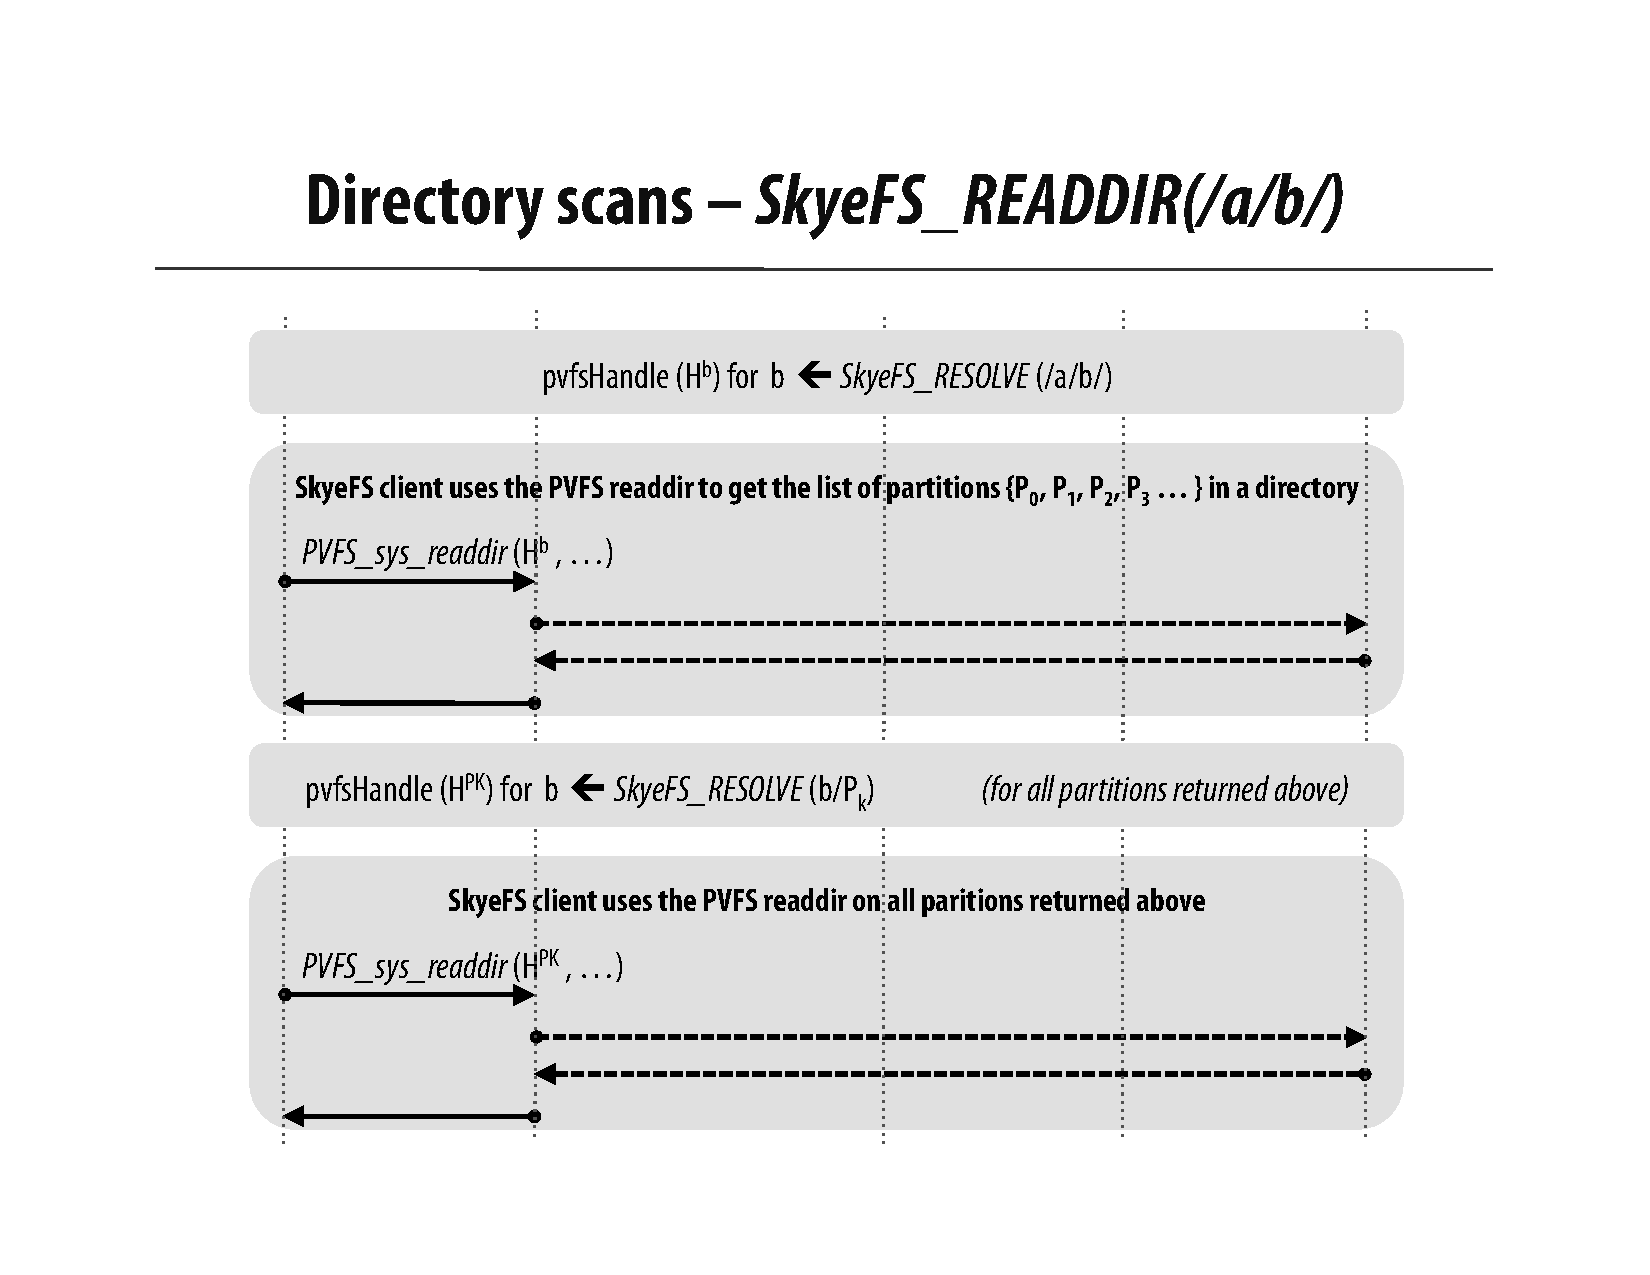
\includegraphics[width=3in]{figure-readdir}
\end{center}
\caption{SkyeFS readdir()}
\end{figure}
The \code{readdir()} operation requires some modification to handle the Giga+
partitioning.  While PVFS provides directory versioning to allow clients to
get a consistent snapshot of a directory we do not provide any such mechanism
to our users.  Instead, our \code{readdir()} mechanism is a ``best effort'' attempt
at providing a listing of the directory.  To accomplish this the client will
perform a \code{PVFS\_sys\_readdir()} of the logical directory handle returned by
\code{lookup()}.  The client will then perform a \code{PVFS\_sys\_readdir()} of all handles
returned aggregating the results.  This naive approach will enter both real
partitions and splitting partitions.  While this may result in some files
being returned twice or not at all it is an inexpensive approach that will
work well in static or small directories.  We anticipate that the directories
for which this approach fails are too big for \code{readdir()} to be useful.

\subsection{Other Operations}
\begin{figure}
\begin{center}
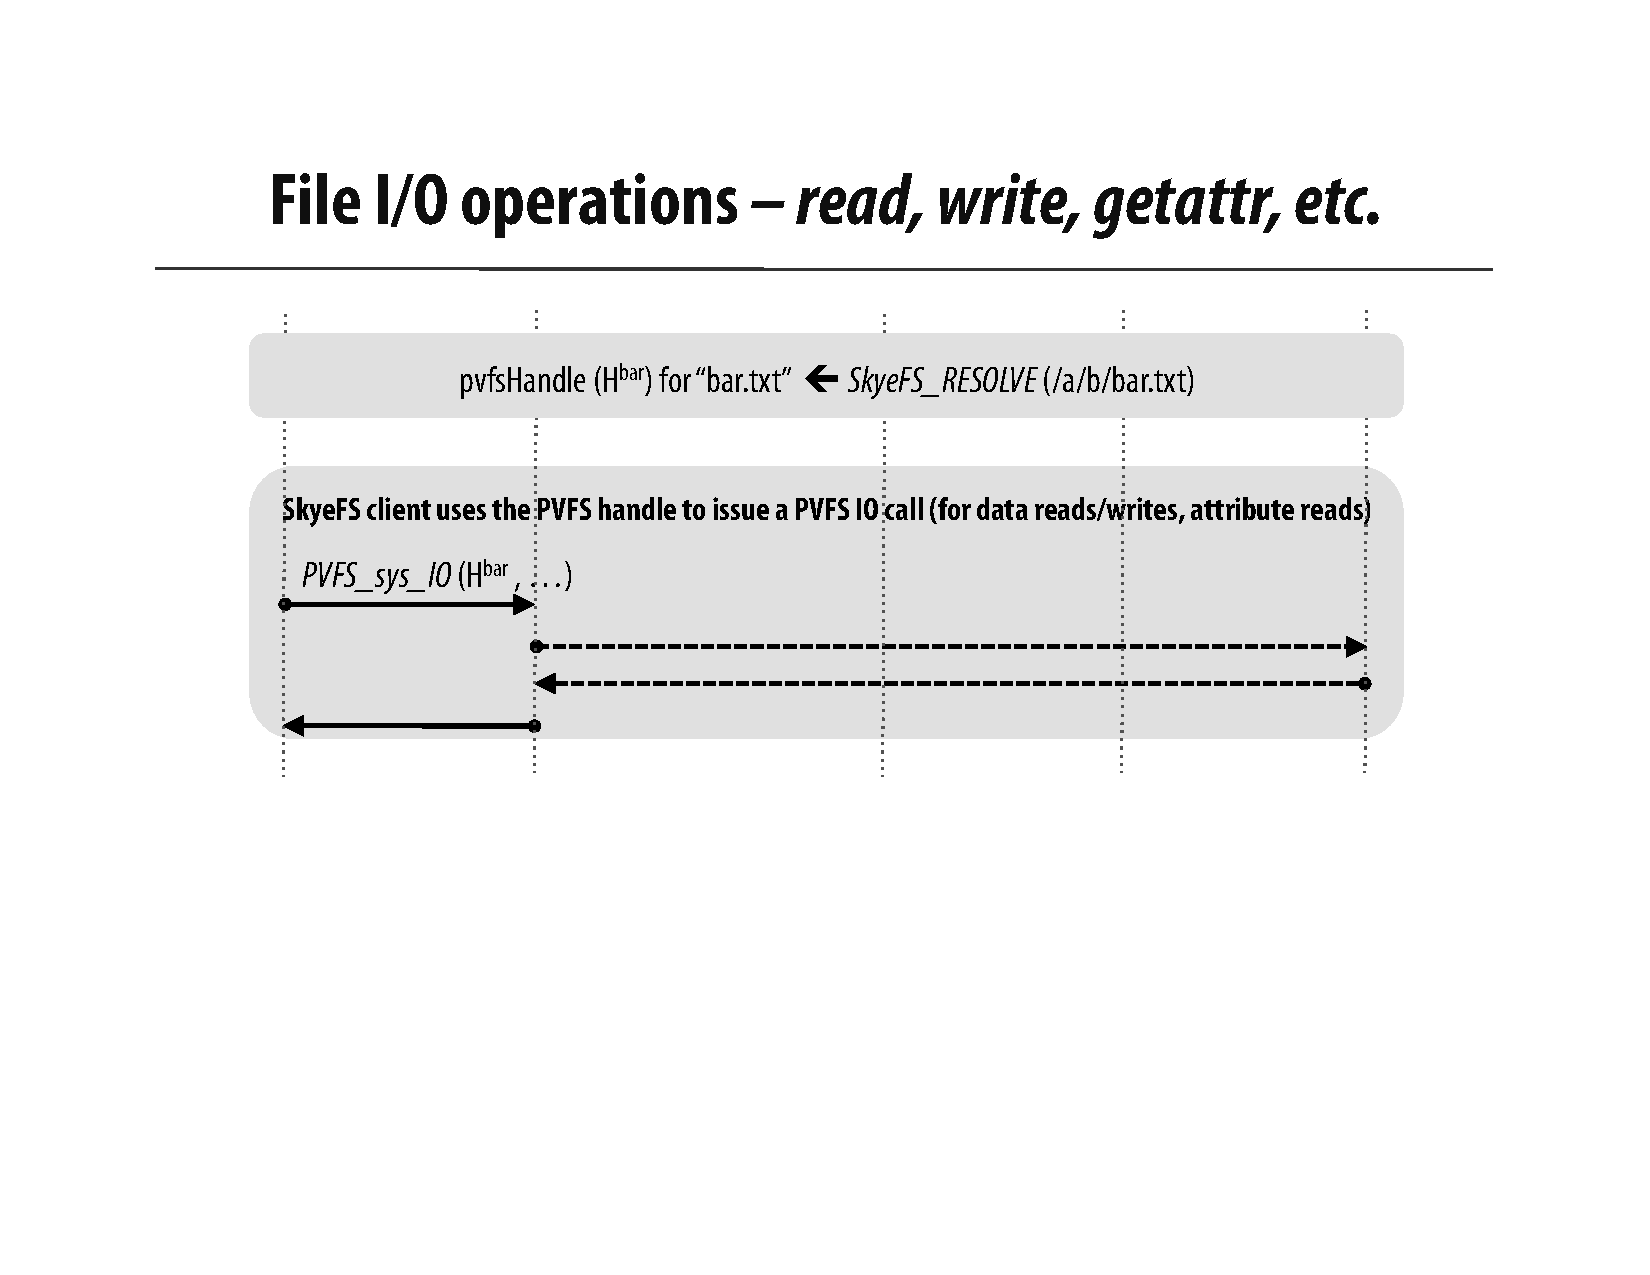
\includegraphics[width=3in]{figure-other}
\end{center}
\caption{SkyeFS IO Operations}
\end{figure}
All other operations are relatively straightforward modifications of their
pvfs2\-fuse counterparts with the PVFS \code{lookup()} operation replaced by
our own version.  This includes both data operations such as \code{read()} and
\code{write()} as well as metadata operations like \code{stat()} and
\code{chmod()}.  Because we resolve all objects to PVFS handles inside their
Giga+ partitions, these operations can proceed on the client without concern
for future splitting.

\section{Other Considerations}
\subsection{Multi-step Lookup}
In the current system, a \code{lookup()} call can only descend one step in a path
traversal.  Future work could extend the operation to provide the entire path
to the \code{skye\_\-server} and allow the server to descend as many
directories in the path as it owns.  This would be of limited value in the
current system where the servers for a parent and child directory are chosen
independently.  At the cost of load balancing, parent and child directories
could be placed often on the same server to allow this mechanism to speed
directory lookups.  One example scheme to achieve this would be to place all
new directories on the same server as their parent.  When a directory splits
the first time the zeroth server would be moved to a new server chosen at
random.  This would have the effect of keeping strings of small (and likely
low-traffic) directories on the same server while still ensuring that large
directories are load-balanced.

\subsection{Server Addition}
PVFS includes very limited support for server addition.  While new servers can
be added to the configuration file for a filesystem and brought online they must
take a previously unoccupied part of the handle space and there exists no
mechanism for automatically migrating either data or metadata to the new server.
The current SkyeFS implementation includes no specific provisions for addition
of servers, however future work could use SkyeFS to support the migration of
some data to new PVFS MDS.  In particular, by splitting overfull but already
load-balanced directories to these new servers some load can be moved to the
servers in already existing directories.  Because SkyeFS stores the number of
servers existing at the time of creation in each directory as an extended
attribute of that directory,\footnote{This is currently unimplemented.} no
specific mechanism is needed to add a new server other than adding the server
to the PVFS cluster and restarting all \code{skye\_\-server} processes.  However,
this mechanism is untested.

\subsection{Fault Tolerance}
PVFS is not a redundant file system and so it has very limited support for fault
tolerant or highly available configurations.  As a result, we do not make any
attempts to provide redundant services or fall over support in the case of
failures.  We assume that \code{skye\_\-server} processes and the PVFS servers fail
together and that any failure will render the system unusable until resolved by
restarting the system.

However, we do make every effort to leave the system in a consistant state at
all times should any component fail.  Any skye process can fail at any time
and the resulting state will be repaired transparently upon restart.  This is
primarily due to the lack of additional SkyeFS metadata that is required on
top of the PVFS file system.  By carefully controlling the sequence of actions
we take on the PVFS file system we are able to ensure that any state of PVFS
is recognizable as either complete or the result of an unfinished action which
can then be resumed or aborted.

\section{Correctness}
To ensure correctness of the system, we tested against a modified version of
Pawel Dawidek's fstest suite.\footnote{Available at
\url{http://people.freebsd.org/~pjd/fstest/}}  Our version was limited to the
tests for \code{chflags}, \code{chmod}, \code{chown}, \code{mkdir},
\code{open}, \code{readdir}, \code{rename}, \code{rmdir} and \code{unlink}.
We removed tests that required hard links, which our filesystem does not
support.

\section{Performance Analysis}

\subsection{Method}
Tests were performed on the Marmot cluster consisting of 128 nodes with two
single core Opteron CPUs, 16GiB of RAM, one SATA disk and Gigabit Ethernet.
PVFS was configured with default settings.  In production configurations, we
expect that PVFS would be run on fast disk arrays.  To prevent the single 7200
RPM disks available from artificially limiting throughput, we ran all
experiments with PVFS configured to use a tmpfs for storage.  In each
experiment, both the clients and servers were located on the same set of
machines

\subsection{File Creation}
\begin{figure}
\begin{center}
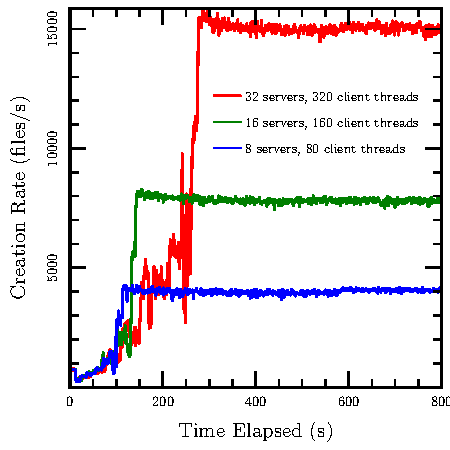
\includegraphics[width=3in]{graph-create}
\end{center}
\caption{SkyeFS Empty File Creation Throughput}
\end{figure}

To test directory insert rates we started with an empty filesystem and created
a single directory.  For each server, we started 10 clients simultaneously
which all attempted to insert uniquely named files into the directory.  We
recorded the overall rate of inserts in the entire system.

For 32 servers, the system reached a peak throughput of over 15k creates per second
after 4 minutes and 30 seconds.  For 16 servers, peak throughput was 8k
creates per second after 2 minutes and 25 seconds.  And for 8 servers, peak
throughput was 4k creates per seconds after 1 minutes and 55 seconds.

This experiment provides the expected linear scaling of throughput after the
system has become load balanced.  We believe the increased time required to
get to a load-balanced state for the 32 server experiment is due to higher
resource contention during the first few splits.  Future work might look at
ways to quicken these first few splits in the event of very high load to
prevent this problem.

We note that the use of FUSE turns each \code{mknod} into a pair of
\code{lookup} and \code{mknod} requests.  The use of the SkyeFS operations
directly, e.g. as part of a shared library, might be able to drastically
improve this performance by avoiding the superfluous \code{lookup}.

\subsection{Readdir}
\begin{figure}
\begin{center}
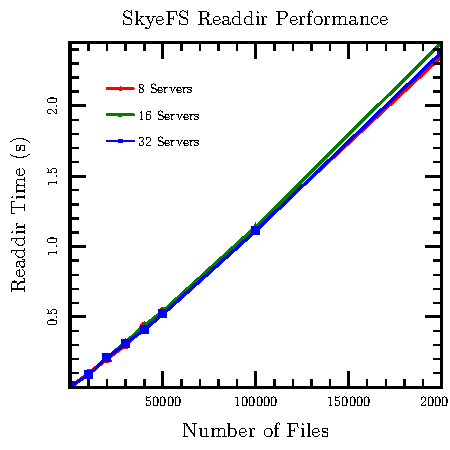
\includegraphics[width=3in]{graph-readdir}
\end{center}
\caption{SkyeFS Readdir Performance}
\end{figure}
One of the desirable properties of the Giga+ algorithm is that it keeps the
overhead for a \code{readdir} small in the case of small directories.  To test
this, we created directories of various sizes and measured the time it took a
single client to read all the entries in the directory.  We repeated this
experiment with 8, 16, and 32 servers.

The client was able to complete a \code{readdir} for a directory with 1000
entries in 0.1 seconds.  As expected, this increased slightly worse than
linearly as the number of entries and partitions increased.  In the case of
200k entries, a \code{readdir} took approximately 2.4 seconds.  No significant
difference in performance was noted between the different server
configurations.

Further work might improve upon this performance by issuing the \code{readdir}
for each partition in parallel.

\subsection{FUSE Low Level API}
Our initial prototype system used the standard FUSE ``high level'' API.  This
API provides a full pathname for every operation.  As a result, each
\code{mknod} call in our file creation experiment required resolving the PVFS
path from the root of the filesystem.  This created an excessive amount of
traffic on the server responsible for the filesystem root and bottlenecked the
system.  We were able to resolve this problem by switching to the lowlevel API
and running our benchmark utility from within the directory in which the files
are to be created.

\subsection{SkyeFS Client and PVFS}
Our initial prototype included a fully multi-threaded client.  However, we
quickly noticed that executing many operations in parallel (for example,
using \code{make -j8} would result in long stalls while executing PVFS calls.
To work around this problem, we currently run the client in the single
threaded FUSE mode.

The FUSE lowlevel API allows the filesystem to return from the callback
without returning a result to FUSE.  After consulting with the PVFS
developers, it has been suggested that using this functionality along with the
asynchronous PVFS operations might allow concurrent operation without
experiencing these stalls.  This was not attempted for this project because of
the large engineering effort required to convert each operation to persist its
state across asynchronous PVFS calls.

\subsection{SkyeFS Server and PVFS}
The \code{skye\_server} is based on the initial Giga+ prototype and uses a
single thread to handle each incoming RPC connection.  As a result, it is easy
for upwards of 100 client operations to be in flight concurrently.  The PVFS
system interface keeps an array of state machines for all outstanding
operations in the address space.  All threads which have an in-flight
operation attempt to take a lock on this array and the thread which acquires
the lock drives progress on all state machines in the array.

The first problem that results from this design is that the array is of
limited size.  Currently, the PVFS code statically defines the array of state
machines to be of length 256.  If an incoming operation would overflow this
array, an assertion is tripped.  To avoid tripping this insertion we
implemented flow control in the form of a semaphore.  When the server starts
the semaphore is initialized to a small value.  When a thread receives an RPC
request, it downs the semaphore before issuing any PVFS requests.  When the
thread completes its work, it will up the semaphore.  In this way, we prevent
more than the semaphore's initial value threads from issuing PVFS requests
concurrently.  In practice, we found that we needed to set this initial value
as low as 32 to avoid tripping the assert.

The other problem with this design is that it does not guarantee fairness to
the requests on the array.  This means that while a request may have
completed, the requesting thread may not notice this for a very long time.
This introduces significant jitter into client response times and slows the
entire system's throughput as a client is unnecessarily blocked on a server
response.  To solve this problem, we further restrict the number of concurrent
operations in flight by initializing our flow control semaphore to 12.
Our testing indicated that this value is optimal in the 32 server case.

\subsection{Split Performance}
During a split the split thread must issue \code{readdir} calls to the
partition which is being split.  While this is happening, additional creates
may be issued against that partition.  We found that without external
synchronization, this pattern of requests results in very poor PVFS
performance.

We wrote a test program to isolate this particular workload.  The program
connects to a provided PVFS server using the system interface.  It then spawns
10 threads which all create files in that directory until 5000 files are
created.  It also spawns another thread that will list out the contents of
that directory repeatedly, reporting the time taken each time.  The program
supports three synchronization models for the threads to test different levels
of interleaving of requests.

In the unsynchronized model all threads are allowed to run without any
synchronization.  On our test system, this required 42 seconds and the
directory listings took between 2 and 12 seconds to complete with a median of
7 seconds.

In our create synchronized model, each of the 10 threads that issue creates
synchronizes on a single mutex such that only one create is every in flight at
a time.  With this model, 41 seconds were required to create the files and the
listings took between 2 and 20 seconds to complete.

In our final, everything synchronized model, all create threads and the
readdir thread synchronized on the same mutex.  With this model, the creates
take 43 seconds to complete and all listings take less than 200ms.
\end{document}
